%Use one of the two documentclass lines depending on aspect ratio needed
% for 4x3 aspect ratio slides
%\documentclass{beamer}
%for 16x9 (modern wide screen) aspect ratio slides
\documentclass[aspectratio=169]{beamer}

% packages
\usepackage{tcolorbox}
\usepackage{graphicx}
\usepackage{tikz}
\usepackage{hyperref}

% Oxford Maths theming
\usetheme{oxfordmaths}

% Set author etc info
\title[EPR Teil II - Jonas] %short version of title for slide footer
{Repetetorium EPI WS 24/25} %full title for titlepage
\author{EPR Teil II - Jonas}
\institute{
Graphen \& Bäume\\
Funktionen, Iteration \& Rekursion\\
NumPy \& Pandas}
\date[28 Februar 2025]  %short date for slide footer
{Rep - 28. Februar} %main date for title page,
                        %can overload it to show say 'Conference X, Date Y'




%% Now for the actual slides %%
\begin{document}

\begin{frame}[plain]
  \titlepage
\end{frame}

\begin{frame}
  \frametitle{Themen}
  \begin{itemize}
      \item Graphen und Bäume
      \item Funktionen in Python
      \item Iteration und Rekursion
      \item Numpy und Pandas
  \end{itemize}
\end{frame}

\begin{frame}{Graphentheorie}
  \begin{columns}
    \hspace*{1cm}\begin{column}{0.64\textwidth}
      \begin{itemize}
        \item Definiert über ein Tupel an Mengen als G = (V,E)
        \begin{itemize}
            \item V: Menge an Knoten (\textit{Vertices})
            \item E: Menge an Kanten (\textit{Edges})
        \end{itemize}
      \end{itemize}
      \pause

      Knoten:
      \begin{itemize}
        \item Elemente/Zustände
      \end{itemize}

      Kanten:
      \begin{itemize}
          \item Verbindungen/Übergänge
      \end{itemize}
    \end{column}
    
    \begin{column}{0.25\textwidth}
      \centering
      \scalebox{0.7}{
        \begin{tikzpicture}[shorten >=1pt, node distance=2cm, auto, 
          every node/.style={circle, draw, fill=blue!20, font=\sffamily}, 
          every edge/.style={draw, thick, blue}]
          
          \node (A) {A};
          \node (B) [right of=A] {B};
          \node (C) [right of=B] {C};
          \node (D) [below of=C] {D};
        
          \path[--]
            (A) edge (B)
            (B) edge (C)
            (C) edge [bend left] (A)
                 edge (D);
          
        \end{tikzpicture}
      }
    \end{column}
  \end{columns}
\end{frame}

\begin{frame}{Graphentheorie}
    \begin{columns}
        \begin{column}{0.5\textwidth}
            \centering \Large Zyklisch (Nicht Kreisfrei)
            \vspace{0.5}
            \begin{figure}[h]
                \centering
                \scalebox{0.9}{
                    \begin{tikzpicture}[shorten >=1pt, node distance=2cm, auto, 
                      every node/.style={circle, draw, fill=blue!20, font=\sffamily}, 
                      every edge/.style={draw, thick, blue}]
                      
                      \node (A) {A};
                      \node (B) [right of=A] {B};
                      \node (C) [right of=B] {C};
                      \node (D) [below of=C] {D};
                    
                      \path[--]
                        (A) edge (B)
                        (B) edge (C)
                        (C) edge [bend left] (A)
                             edge (D);
                      
                    \end{tikzpicture}
                }
            \end{figure}
        \end{column}
        \pause
        \vline
        \begin{column}{0.5\textwidth}
            \centering \Large Azyklisch (Kreisfrei)
            \vspace{0.75cm}
            \begin{figure}[h]
                \centering
                \scalebox{0.9}{ % Adjust scale here
                    \begin{tikzpicture}[shorten >=1pt, node distance=2cm, auto, 
                    every node/.style={circle, draw, fill=blue!20, font=\sffamily}, 
                    every edge/.style={draw, thick, blue}]
                    
                    \node (A) {A};
                    \node (B) [right of=A] {B};
                    \node (C) [right of=B] {C};
                    \node (D) [right of=C] {D};
                    
                    \path[--]
                        (A) edge (B)
                        (B) edge (C)
                        (C) edge (D);
                    
                    \end{tikzpicture}
                }
            \end{figure}
            \vspace{0.75cm}
        \end{column}
    \end{columns}
\end{frame}

\begin{frame}{Graphentheorie}
    \begin{columns}
        \begin{column}{0.5\textwidth}
            \centering \Large Zusammenhängend
            \vspace{0.75cm}
            \begin{figure}[h]
                \centering
                \scalebox{0.9}{ % Adjust scale here
                    \begin{tikzpicture}[shorten >=1pt, node distance=2cm, auto, 
                    every node/.style={circle, draw, fill=blue!20, font=\sffamily}, 
                    every edge/.style={draw, thick, blue}]
                    
                    \node (A) {A};
                    \node (B) [right of=A] {B};
                    \node (C) [right of=B] {C};
                    \node (D) [right of=C] {D};
                    
                    \path[--]
                        (A) edge (B)
                        (B) edge (C)
                        (C) edge (D);
                    
                    \end{tikzpicture}
                }
            \end{figure}
            \vspace{0.75cm}
        \end{column}
        \pause
        \vline
        \begin{column}{0.5\textwidth}
            \centering \Large Nicht Zusammenhängend
            \begin{figure}[h]
                \centering
                \scalebox{0.9}{ % Adjust scale here
                    \begin{tikzpicture}[shorten >=1pt, node distance=2cm, auto, 
                        every node/.style={circle, draw, fill=blue!20, font=\sffamily}, 
                        every edge/.style={draw, thick, blue}]
                        
                        \node (A) {A};
                        \node (B) [right of=A] {B};
                        \node (C) [right of=B] {C};
                        \node (D) [below of=B, xshift=2cm] {D}; % Place D separately
                        
                        \path[--]
                            (A) edge (B)
                            (B) edge (C);
                        
                    \end{tikzpicture}
                }
            \end{figure}
        \end{column}
    \end{columns}
\end{frame}

\begin{frame}{Graphentheorie}
    \vspace{0.5cm}
    \begin{columns}
        \begin{column}{0.5\textwidth}
            \centering \Large Ungerichtet \normalsize
            \begin{figure}[h]
            \centering
            \scalebox{0.7}{ % Adjust scale here
                \begin{tikzpicture}[shorten >=1pt, node distance=2cm, auto, 
                    every node/.style={circle, draw, fill=blue!20, font=\sffamily}, 
                    every edge/.style={draw, thick, blue}]
                    
                    \node (A) {A};
                    \node (B) [right of=A] {B};
                    \node (C) [right of=B] {C};
                    \node (D) [right of=C] {D};
                    \node (E) [right of=D] {E};
                    
                    \path[--]
                        (A) edge (B)
                        (B) edge (C)
                        (C) edge (D)
                        (D) edge (E)
                        (E) edge [bend left] (A)
                    
                \end{tikzpicture}
            }
            \end{figure}
        \end{column}
        \vline
        \begin{column}{0.5\textwidth}
            \centering \Large Gerichtet \normalsize
            \begin{figure}[h]
            \centering
            \scalebox{0.7}{ % Adjust scale here
                \begin{tikzpicture}[shorten >=1pt, node distance=2cm, auto, 
                    every node/.style={circle, draw, fill=blue!20, font=\sffamily}, 
                    every edge/.style={draw, thick, blue}]
                    
                    \node (A) {A};
                    \node (B) [right of=A] {B};
                    \node (C) [right of=B] {C};
                    \node (D) [right of=C] {D};
                    \node (E) [right of=D] {E};
                    
                    \path[->]
                        (A) edge (B)
                        (B) edge (C)
                        (C) edge (D)
                        (D) edge (E)
                        (E) edge [bend left] (A)
                    
                \end{tikzpicture}
            }
            \end{figure}
        \end{column}
    \end{columns}
\end{frame}

\begin{frame}{Graphentheorie}
    \vspace{0.5cm}
    \begin{columns}
        \begin{column}{0.5\textwidth}
            \centering \Large Adjazenzliste \normalsize
            \begin{itemize}
                \item Liste aller Adjazenzknoten eines Knotens
            \end{itemize}
            \begin{table}[]
                \centering
                \begin{tabular}{c|c}
                    A & \{A, C\} \\
                    B & \{A, B\} \\
                    C & $\emptyset$
                \end{tabular}
            \end{table}
        \end{column}
        \pause
        \vline
        \begin{column}{0.5\textwidth}
            \centering \Large Adjazenzmatrix \normalsize
            \begin{itemize}
                \item $n \times n$ - Matrix
            \end{itemize}
            \begin{table}[]
                \centering
                \begin{tabular}{c|c c c}
                     & A & B & C \\
                     \hline
                    A & 1 & 0 & 1 \\
                    B & 1 & 1 & 0 \\
                    C & 0 & 0 & 0 \\
                \end{tabular}
            \end{table}
        \end{column}
    \end{columns}
    \vspace{0.5cm}
    \pause
    \centering Beide Darstellungen repräsentieren den gleichen Graphen
\end{frame}
% Azyklisch oder nicht?
\begin{frame}{Graphentheorie}
    \vspace{0.5cm}
    \begin{columns}
        \begin{column}{0.5\textwidth}
            \centering \Large Adjazenzliste \normalsize
            \begin{table}[]
                \centering
                \begin{tabular}{c|c}
                    A & \{A, C\} \\
                    B & \{A, B\} \\
                    C & $\emptyset$
                \end{tabular}
            \end{table}
        \end{column}
        \pause
        \begin{column}{0.5\textwidth}
            \begin{figure}[h]
            \centering
            \scalebox{1.2}{ % Adjust scale here
                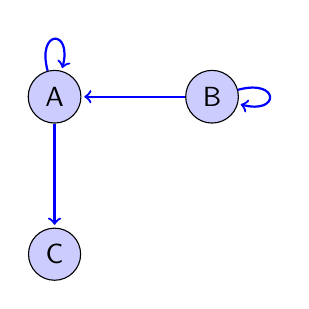
\begin{tikzpicture}[shorten >=1pt, node distance=2cm, auto, 
                every node/.style={circle, draw, fill=blue!20, font=\sffamily}, 
                every edge/.style={draw, thick, blue}]
                
                \node (A) {A};
                \node (B) [right of=A] {B};
                \node (C) [below of=A] {C};
                
                \path[->]
                    (A) edge [loop above] (A) % Loop at A
                    (A) edge (C) % Edge from A to C
                    (B) edge (A) % Edge from B to A
                    (B) edge [loop right] (B); % Loop at B
                
                \end{tikzpicture}
            }
        \end{figure}
        \end{column}
    \end{columns}
\end{frame}

\begin{frame}{Graphentheorie}
    \vspace{0.5cm}
    \begin{columns}
        \begin{column}{0.5\textwidth}
            \centering \Large Adjazenzmatrix \normalsize
            \begin{table}[]
                \centering
                \begin{tabular}{c|c c c}
                     & A & B & C \\
                     \hline
                    A & 1 & 0 & 1 \\
                    B & 1 & 1 & 0 \\
                    C & 0 & 0 & 0 \\
                \end{tabular}
            \end{table}
        \end{column}
        \pause
        \begin{column}{0.5\textwidth}
            \begin{figure}[h]
            \centering
            \scalebox{1.2}{ % Adjust scale here
                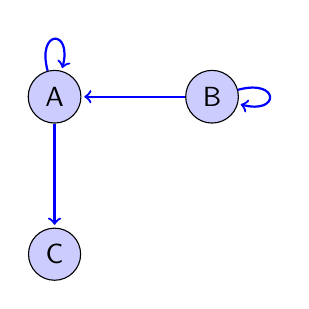
\begin{tikzpicture}[shorten >=1pt, node distance=2cm, auto, 
                every node/.style={circle, draw, fill=blue!20, font=\sffamily}, 
                every edge/.style={draw, thick, blue}]
                
                \node (A) {A};
                \node (B) [right of=A] {B};
                \node (C) [below of=A] {C};
                
                \path[->]
                    (A) edge [loop above] (A) % Loop at A
                    (A) edge (C) % Edge from A to C
                    (B) edge (A) % Edge from B to A
                    (B) edge [loop right] (B); % Loop at B
                
                \end{tikzpicture}
            }
        \end{figure}
        \end{column}
    \end{columns}
\end{frame}

\begin{frame}{Graphentheorie}
    \vspace{0.5cm}
    \begin{columns}
        \begin{column}{0.5\textwidth}
            \centering \Large Adjazenzliste \normalsize
            \begin{table}[]
                \centering
                \begin{tabular}{c|c}
                    A & \{A, C\} \\
                    B & \{A, B\} \\
                    C & $\emptyset$
                \end{tabular}
            \end{table}
        \end{column}
        \begin{column}{0.5\textwidth}
            \centering \Large Programmatische Umsetzung \normalsize
            \pause
            \begin{tcolorbox}[colframe=oxfordblue, colback=blue!10, coltitle=white, title=Python]
                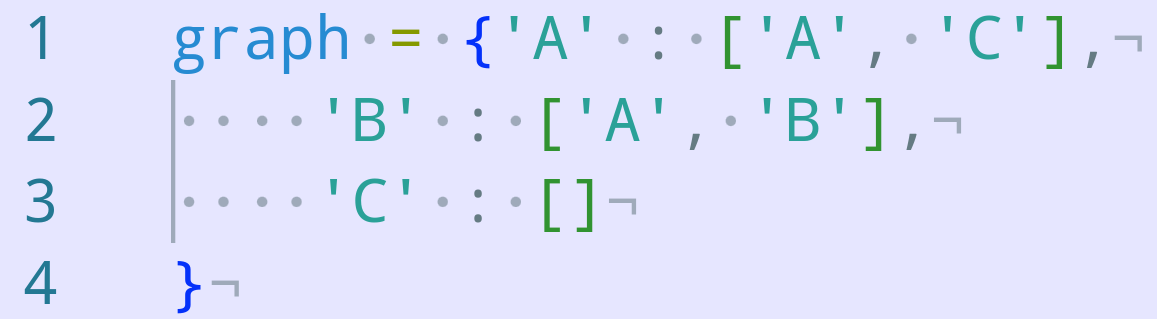
\includegraphics[width=\textwidth]{images/code_adjazenzliste.png}
            \end{tcolorbox}
        \end{column}
    \end{columns}
\end{frame}

\begin{frame}{Graphentheorie}
    \vspace{0.5cm}
    \begin{columns}
        \begin{column}{0.5\textwidth}
            \centering \Large Adjazenzmatrix \normalsize
            \begin{table}[]
                \centering
                \begin{tabular}{c|c c c}
                     & A & B & C \\
                     \hline
                    A & 1 & 0 & 1 \\
                    B & 1 & 1 & 0 \\
                    C & 0 & 0 & 0 \\
                \end{tabular}
            \end{table}
        \end{column}
        \begin{column}{0.5\textwidth}
            \centering \Large Programmatische Umsetzung \normalsize
            \begin{itemize}
                \item Zweidimensionale verschachtelte Liste oder \textit{nested list}
                \item Speicherplatz ist \textit{quaddratisch} im Vergleich zu \textit{linear} bei Adjazenzlisten, daher unüblich
            \end{itemize}
        \end{column}
    \end{columns}
\end{frame}

\begin{frame}{Graphentheorie}
    \Large Komplexeres Beispiel \normalsize
    \vspace{0.5cm}
    \begin{columns}
        \begin{column}{0.4\textwidth}
            \begin{itemize}
                \item Adjazenzmatrix
                \begin{table}[]
                    \centering
                    \begin{tabular}{c|c c c c c c}
                         & A & B & C & D & E & F \\
                         \hline
                        A & 0 & 0 & 1 & 0 & 0 & 0 \\
                        B & 0 & 0 & 1 & 0 & 1 & 0 \\
                        C & 1 & 1 & 0 & 1 & 1 & 0 \\
                        D & 0 & 0 & 1 & 0 & 0 & 0 \\
                        E & 0 & 1 & 1 & 0 & 0 & 0 \\
                        F & 0 & 0 & 0 & 0 & 0 & 0 \\
                    \end{tabular}
                \end{table}
            \end{itemize}
        \end{column}
        \pause
        \begin{column}{0.3\textwidth}
            \begin{itemize}
                \item Adjazenzliste
                \begin{table}[]
                    \centering
                    \begin{tabular}{c|c}
                        A & \{C\} \\
                        B & \{C, E\} \\
                        C & \{A, B, D, E\} \\
                        D & \{C\} \\
                        E & \{B, C\} \\
                        F & $\emptyset$ \\
                    \end{tabular}
                \end{table}
            \end{itemize}
                \vspace{0.25cm}
        \end{column}
        \pause
        \begin{column}{0.3\textwidth}
            \begin{figure}[h]
            \centering
            \scalebox{1.0}{ % Adjust scale here
                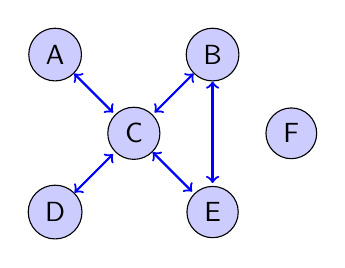
\begin{tikzpicture}[shorten >=1pt, node distance=2cm, auto, 
                every node/.style={circle, draw, fill=blue!20, font=\sffamily}, 
                every edge/.style={draw, thick, blue}]

                \node[shape=circle,draw=black] (A) at (-1,1) {A};
                \node[shape=circle,draw=black] (B) at (1,1) {B};
                \node[shape=circle,draw=black] (C) at (0,0) {C};
                \node[shape=circle,draw=black] (D) at (-1,-1) {D};
                \node[shape=circle,draw=black] (E) at (1,-1) {E};
                \node[shape=circle,draw=black] (F) at (2,0) {F} ;
            
                \path [<->](A) edge (C);
                \path [<->](B) edge (C);
                \path [<->](B) edge (E);
                \path [<->](C) edge (E);
                \path [<->](D) edge (C);
            \end{tikzpicture}
            }
            \end{figure}
        \end{column}
    \end{columns}
\end{frame}

\begin{frame}{Graphentheorie}
    Grundbegriffe \textit{(Recap)}
    \begin{itemize}
        \item Knoten: Element/Zustand
        \pause
        \item Kante: Verbindung/Übergang
        \pause
        \item Grad: Anzahl an Kanten die den Knoten verbinden (nur wenn ungerichtet)
        \pause
        \item Eingangsgrad: Anzahl an Kanten die in den Knoten zeigen (nur wenn gerichtet)
        \pause
        \item Ausgangsgrad: Anzahl an Kanten die aus dem Knoten zeigen (nur wenn gerichtet)
        \pause
        \item Adjazenzliste: Liste an Knoten die durch den Knoten erreicht werden
        \pause
        \item Adjazenzmatrix: Matrix mit \texttt{boolean}-Wert für jede Knoten-Verbindung
        \pause
        \item Zusammenhängend: Jeder Knoten kann von kedem Knoten erreicht werden (nur wenn ungerichtet)
        \pause
        \item Schwach zusammenhängend: alle Knoten sind über mindestens eine Kante verbunden (nur wenn gerichtet)
        \item Stark zusammenhängend: man kann von allen zu allen Knoten und zurück (nur wenn gerichtet)
    \end{itemize}
\end{frame}

\begin{frame}{Graphentheorie}
    \textbf{Baum} - Spezialfall von Graphen
    \begin{columns}
        \begin{column}{0.7\textwidth}
            \begin{itemize}
                \item azyklisch
                \pause
                \item $n - 1$ Kanten bei $n$ Knoten
                \pause
                \item Innerer Knoten: Knoten der weder Wurzel noch Blatt ist
                \pause
                \item Tiefe: Pfadlänge (Anzahl an Kanten) von der Wurzel zum Knoten
                \pause
                \item Höhe: Pfadlänge (Anzahl an Kanten) vom Knoten zum nächsten Blatt
                \pause
                \item Eltern: Vorgänger
                \pause
                \item Kinder: Nachfahren
                \pause
                \item Geschwister: Knoten mit gleichem Elternknoten
            \end{itemize}
        \end{column}
        \begin{column}{0.3\textwidth}
            \begin{figure}[h]
            \centering
            \onslide
            \scalebox{0.5}{ % Adjust scale here
                \begin{tikzpicture}[shorten >=1pt, node distance=2cm, auto, 
                every node/.style={circle, draw, fill=blue!20, font=\sffamily}, 
                every edge/.style={draw, thick, blue}]
        
                % Define nodes
                \node[shape=circle,draw=black] (A) at (0,2) {A}; % Root node
                \node[shape=circle,draw=black] (B) at (-2,1) {B}; % Child of A
                \node[shape=circle,draw=black] (C) at (2,1) {C}; % Child of A
                \node[shape=circle,draw=black] (D) at (-3,0) {D}; % Child of B
                \node[shape=circle,draw=black] (E) at (-1,0) {E}; % Child of B
                \node[shape=circle,draw=black] (F) at (1,0) {F}; % Child of C
        
                % Define edges
                \path [--](A) edge (B);
                \path [--](A) edge (C);
                \path [--](B) edge (D);
                \path [--](B) edge (E);
                \path [--](C) edge (F);
                \end{tikzpicture}
            }
            \end{figure}
        \end{column}
    \end{columns}
\end{frame}


\begin{frame}{Graphentheorie}
    \textbf{Ungerichteter Baum}
    \begin{columns}
        \begin{column}{0.7\textwidth}
            \begin{itemize}
            \pause
                \item zusammenhängend
                \pause
                \item Wurzel: "Hauptknoten" (kann beliebig ausgewählt werden)
                \pause
                \item Blatt: Knoten ohne Nachfolger
                \pause
                \item Ordnung: maximaler Grad - 1
            \end{itemize}
        \end{column}
        \begin{column}{0.3\textwidth}
            \begin{figure}[h]
            \centering
            \onslide
            \scalebox{0.5}{ % Adjust scale here
                \begin{tikzpicture}[shorten >=1pt, node distance=2cm, auto, 
                every node/.style={circle, draw, fill=blue!20, font=\sffamily}, 
                every edge/.style={draw, thick, blue}]
        
                % Define nodes
                \node[shape=circle,draw=black] (A) at (0,2) {A}; % Root node
                \node[shape=circle,draw=black] (B) at (-2,1) {B}; % Child of A
                \node[shape=circle,draw=black] (C) at (2,1) {C}; % Child of A
                \node[shape=circle,draw=black] (D) at (-3,0) {D}; % Child of B
                \node[shape=circle,draw=black] (E) at (-1,0) {E}; % Child of B
                \node[shape=circle,draw=black] (F) at (1,0) {F}; % Child of C
                \node[shape=circle,draw=black] (G) at (3,0) {G}; % Child of C
        
                % Define edges
                \path [--](A) edge (B);
                \path [--](A) edge (C);
                \path [--](B) edge (D);
                \path [--](B) edge (E);
                \path [--](C) edge (F);
                \path [--](C) edge (G);
                \end{tikzpicture}
            }
            \end{figure}
        \end{column}
    \end{columns}
\end{frame}

\begin{frame}{Graphentheorie}
    \textbf{Gerichteter Baum}
    \begin{columns}
        \begin{column}{0.7\textwidth}
            \begin{itemize}
            \pause
                \item nicht zusammenhängend
                \pause
                \item Wurzel: Knoten mit Eingangsgrad 0
                \pause
                \item Blatt: Knoten mit Ausgangsgrad 0
                \pause
                \item Ordnung: maximaler Ausgangsgrad
            \end{itemize}
        \end{column}
        \begin{column}{0.3\textwidth}
            \begin{figure}[h]
            \centering
            \onslide
            \scalebox{0.5}{ % Adjust scale here
                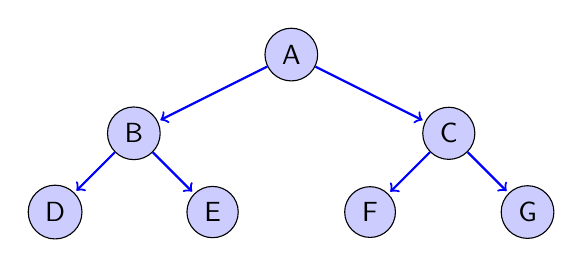
\begin{tikzpicture}[shorten >=1pt, node distance=2cm, auto, 
                every node/.style={circle, draw, fill=blue!20, font=\sffamily}, 
                every edge/.style={draw, thick, blue}]
        
                % Define nodes
                \node[shape=circle,draw=black] (A) at (0,2) {A}; % Root node
                \node[shape=circle,draw=black] (B) at (-2,1) {B}; % Child of A
                \node[shape=circle,draw=black] (C) at (2,1) {C}; % Child of A
                \node[shape=circle,draw=black] (D) at (-3,0) {D}; % Child of B
                \node[shape=circle,draw=black] (E) at (-1,0) {E}; % Child of B
                \node[shape=circle,draw=black] (F) at (1,0) {F}; % Child of C
                \node[shape=circle,draw=black] (G) at (3,0) {G}; % Child of C
        
                % Define edges
                \path [->](A) edge (B);
                \path [->](A) edge (C);
                \path [->](B) edge (D);
                \path [->](B) edge (E);
                \path [->](C) edge (F);
                \path [->](C) edge (G);
                \end{tikzpicture}
            }
            \end{figure}
        \end{column}
    \end{columns}
\end{frame}

\begin{frame}{Graphentheorie}
    \textbf{Spezielle Bäume I}
    \begin{columns}
        \begin{column}{0.5\textwidth}
            \begin{itemize}
                \item Binärbaum
                \begin{itemize}
                    \item 0 - 2  Kinder
                    \item Eindeutiger Unterschied zwischen linkem und rechten Kind
                \end{itemize}
            \end{itemize}
        \end{column}
        \begin{column}{0.5\textwidth}
            \begin{figure}[h]
                \centering
                \onslide
                \scalebox{0.7}{ % Adjust scale here
                    \begin{tikzpicture}[shorten >=1pt, node distance=2cm, auto, 
                        every node/.style={circle, draw, fill=blue!20, font=\sffamily}, 
                        every edge/.style={draw, thick, blue}]
                
                        % Define nodes
                        \node[shape=circle,draw=black] (1) at (0,2) {1}; % Root node
                        \node[shape=circle,draw=black] (2) at (-2,1) {2}; % Child of A
                        \node[shape=circle,draw=black] (3) at (2,1) {3}; % Child of A
                        \node[shape=circle,draw=black] (4) at (-3,0) {4}; % Child of B
                        \node[shape=circle,draw=black] (5) at (-1,0) {5}; % Child of B
                        \node[shape=circle,draw=black] (6) at (1,0) {6}; % Child of C
                
                        % Define edges
                        \path [->](1) edge (2);
                        \path [->](1) edge (3);
                        \path [->](2) edge (4);
                        \path [->](2) edge (E);
                        \path [->](3) edge (F);
                    \end{tikzpicture}
                }
            \end{figure}
            \centering \LARGE $\neq$ \normalsize
            \begin{figure}[h]
                \centering
                \onslide
                \scalebox{0.7}{ % Adjust scale here
                    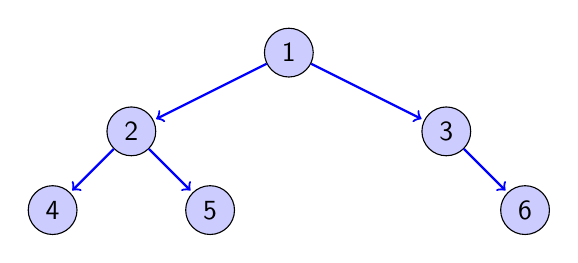
\begin{tikzpicture}[shorten >=1pt, node distance=2cm, auto, 
                        every node/.style={circle, draw, fill=blue!20, font=\sffamily}, 
                        every edge/.style={draw, thick, blue}]
                
                        % Define nodes
                        \node[shape=circle,draw=black] (A) at (0,2) {1}; % Root node
                        \node[shape=circle,draw=black] (B) at (-2,1) {2}; % Child of A
                        \node[shape=circle,draw=black] (C) at (2,1) {3}; % Child of A
                        \node[shape=circle,draw=black] (D) at (-3,0) {4}; % Child of B
                        \node[shape=circle,draw=black] (E) at (-1,0) {5}; % Child of B
                        \node[shape=circle,draw=black] (F) at (3,0) {6}; % Child of C
                
                        % Define edges
                        \path [->](A) edge (B);
                        \path [->](A) edge (C);
                        \path [->](B) edge (D);
                        \path [->](B) edge (E);
                        \path [->](C) edge (F);
                        \end{tikzpicture}
                    }
                \end{figure}
        \end{column}
    \end{columns}
\end{frame}

\begin{frame}{Graphentheorie}
    \textbf{Spezielle Bäume II}
    \begin{columns}
        \begin{column}{0.5\textwidth}
            \begin{itemize}
                \item Balancierter Baum
                \begin{itemize}
                    \item die Länge der Pfade von der Wurzel zu allen Blättern darf sich um höchstens 1 unterscheiden
                \end{itemize}
            \end{itemize}
        \end{column}
        \begin{column}{0.5\textwidth}
        \centering \large balanciert \normalsize
            \begin{figure}[h]
                \centering
                \onslide
                \scalebox{0.6}{ % Adjust scale here
                    \begin{tikzpicture}[shorten >=1pt, node distance=2cm, auto, 
                        every node/.style={circle, draw, fill=blue!20, font=\sffamily}, 
                        every edge/.style={draw, thick, blue}]
                
                        % Define nodes
                        \node[shape=circle,draw=black] (1) at (0,2) {1}; % Root node
                        \node[shape=circle,draw=black] (2) at (-2,1) {2}; % Child of A
                        \node[shape=circle,draw=black] (3) at (2,1) {3}; % Child of A
                        \node[shape=circle,draw=black] (4) at (-3,0) {4}; % Child of B
                        \node[shape=circle,draw=black] (5) at (-1,0) {5}; % Child of B
                
                        % Define edges
                        \path [->](1) edge (2);
                        \path [->](1) edge (3);
                        \path [->](2) edge (4);
                        \path [->](2) edge (E);
                    \end{tikzpicture}
                }
            \end{figure}
            \begin{figure}[h]
                \centering
                \scalebox{0.6}{ % Adjust scale here
                    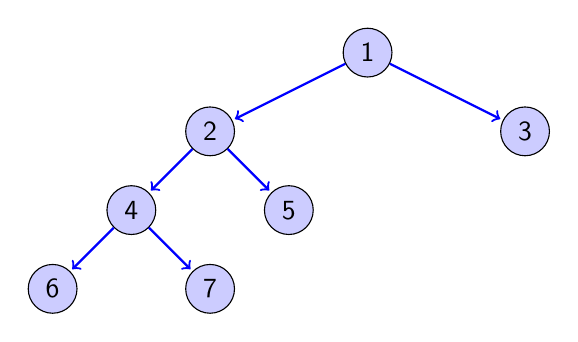
\begin{tikzpicture}[shorten >=1pt, node distance=2cm, auto, 
                        every node/.style={circle, draw, fill=blue!20, font=\sffamily}, 
                        every edge/.style={draw, thick, blue}]
                    
                        % Define nodes
                        \node[shape=circle,draw=black] (A) at (0,3) {1}; % Root node
                        \node[shape=circle,draw=black] (B) at (-2,2) {2}; % Child of A
                        \node[shape=circle,draw=black] (C) at (2,2) {3}; % Child of A
                        \node[shape=circle,draw=black] (D) at (-3,1) {4}; % Child of B
                        \node[shape=circle,draw=black] (E) at (-1,1) {5}; % Child of B
                        \node[shape=circle,draw=black] (F) at (-4,0) {6}; % Child of C
                        \node[shape=circle,draw=black] (G) at (-2,0) {7}; % Child of F
            
                        % Define edges
                        \path [->](A) edge (B);
                        \path [->](A) edge (C);
                        \path [->](B) edge (D);
                        \path [->](B) edge (E);
                        \path [->](D) edge (F);
                        \path [->](D) edge (G);
                    \end{tikzpicture}
                }
            \end{figure}
            \centering \large nicht balanciert \normalsize
        \end{column}
    \end{columns}
\end{frame}

\begin{frame}{Graphentheorie}
    \vspace{-1.7cm}
    \textbf{Spezielle Bäume III}
    \begin{columns}
        \begin{column}{0.5\textwidth}
            \begin{itemize}
                \item Suchbaum
                \begin{itemize}
                    \item geordnete Knoten zum schnelleren Finden von Elementen
                \end{itemize}
            \end{itemize}
        \end{column}
        \begin{column}{0.5\textwidth}
            \begin{figure}[h]
            \centering
            \scalebox{0.8}{ % Adjust scale here
                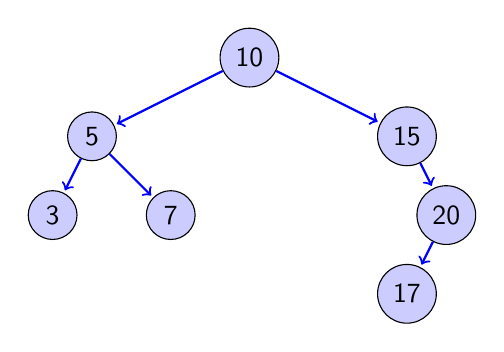
\begin{tikzpicture}[shorten >=1pt, node distance=2cm, auto, 
                    every node/.style={circle, draw, fill=blue!20, font=\sffamily}, 
                    every edge/.style={draw, thick, blue}]
                
                    % Define nodes (changed to fit the binary search tree property)
                    \node[shape=circle,draw=black] (A) at (0,3) {10}; % Root node
                    \node[shape=circle,draw=black] (B) at (-2,2) {5}; % Child of A
                    \node[shape=circle,draw=black] (C) at (2,2) {15}; % Child of A
                    \node[shape=circle,draw=black] (D) at (-2.5,1) {3}; % Child of B
                    \node[shape=circle,draw=black] (E) at (-1,1) {7}; % Child of B
                    \node[shape=circle,draw=black] (F) at (2.5,1) {20}; % Child of C
                    \node[shape=circle,draw=black] (G) at (2,0) {17}; % Child of F
        
                    % Define edges
                    \path [->](A) edge (B);
                    \path [->](A) edge (C);
                    \path [->](B) edge (D);
                    \path [->](B) edge (E);
                    \path [->](C) edge (F);
                    \path [->](F) edge (G);
                \end{tikzpicture}
            }
        \end{figure}
        \end{column}
    \end{columns}
\end{frame}

\begin{frame}{Graphentheorie}
    \begin{columns}
        \begin{column}{0.5\textwidth}
            \textbf{Spezielle Bäume IV}
            \begin{itemize}
                \item HEAP (Heap-Eigenschaft)
                \begin{itemize}
                    \item Die traversierten Knoten jedes Pfades von der Wurzel zu den Blättern ist auf-/ oder absteigend
                \end{itemize}
                \begin{itemize}
                    \item Min-Heap: in aufsteigender Reihenfolge (Wurzel $\rightarrow$ Blatt)
                    \item Max-Heap: in absteigender Reihenfolge (Wurzel $\rightarrow$ Blatt)
                \end{itemize}
            \end{itemize}
        \end{column}
        \begin{column}{0.5\textwidth}
            \begin{figure}[h]
                \centering
                \scalebox{0.7}{ % Adjust scale here
                    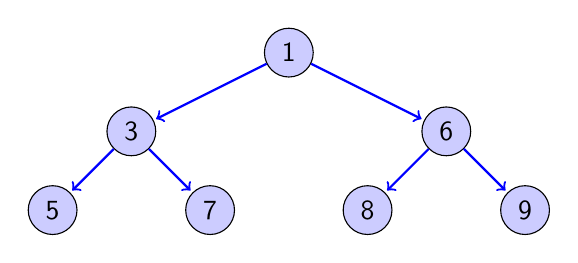
\begin{tikzpicture}[shorten >=1pt, node distance=2cm, auto, 
                        every node/.style={circle, draw, fill=blue!20, font=\sffamily}, 
                        every edge/.style={draw, thick, blue}]
                    
                        % Min-Heap
                        \node[shape=circle,draw=black] (A) at (0,3) {1}; % Root node
                        \node[shape=circle,draw=black] (B) at (-2,2) {3}; % Child of A
                        \node[shape=circle,draw=black] (C) at (2,2) {6}; % Child of A
                        \node[shape=circle,draw=black] (D) at (-3,1) {5}; % Child of B
                        \node[shape=circle,draw=black] (E) at (-1,1) {7}; % Child of B
                        \node[shape=circle,draw=black] (F) at (1,1) {8}; % Child of C
                        \node[shape=circle,draw=black] (G) at (3,1) {9}; % Child of C
            
                        % Define edges
                        \path [->](A) edge (B);
                        \path [->](A) edge (C);
                        \path [->](B) edge (D);
                        \path [->](B) edge (E);
                        \path [->](C) edge (F);
                        \path [->](C) edge (G);
                    \end{tikzpicture}
                }
            \end{figure}
            \centering Min-Heap Eigenschafft erfüllt
            \begin{figure}[h]
                \centering
                \scalebox{0.7}{ % Adjust scale here
                    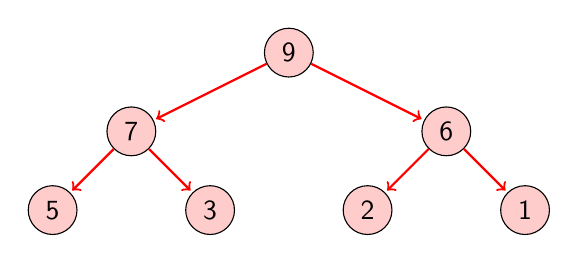
\begin{tikzpicture}[shorten >=1pt, node distance=2cm, auto, 
                        every node/.style={circle, draw, fill=red!20, font=\sffamily}, 
                        every edge/.style={draw, thick, red}]
                    
                        % Max-Heap
                        \node[shape=circle,draw=black] (A) at (0,3) {9}; % Root node
                        \node[shape=circle,draw=black] (B) at (-2,2) {7}; % Child of A
                        \node[shape=circle,draw=black] (C) at (2,2) {6}; % Child of A
                        \node[shape=circle,draw=black] (D) at (-3,1) {5}; % Child of B
                        \node[shape=circle,draw=black] (E) at (-1,1) {3}; % Child of B
                        \node[shape=circle,draw=black] (F) at (1,1) {2}; % Child of C
                        \node[shape=circle,draw=black] (G) at (3,1) {1}; % Child of C
            
                        % Define edges
                        \path [->](A) edge (B);
                        \path [->](A) edge (C);
                        \path [->](B) edge (D);
                        \path [->](B) edge (E);
                        \path [->](C) edge (F);
                        \path [->](C) edge (G);
                    \end{tikzpicture}
                }
            \end{figure}
            \centering Max-Heap Eigenschafft erfüllt
        \end{column}
    \end{columns}
\end{frame}

\begin{frame}{Graphentheorie}
    \vspace{-1.7cm}
    \textbf{Traversierung}
    \begin{columns}
        \begin{column}{0.5\textwidth}
            \begin{itemize}
                \item Es gibt 3 Arten einen Baum zu traversieren:
                \begin{itemize}
                    \item Pre-Order
                    \item In-Order
                    \item Post-Order
                \end{itemize}
                \pause
                \item Bei der Traversierung werden alle Knoten in der erreichten Reihenfolge aufgeschrieben
            \end{itemize}
        \end{column}
        \onslide
        \begin{column}{0.5\textwidth}
            \begin{figure}[h]
            \centering
            \scalebox{1}{ % Adjust scale here
                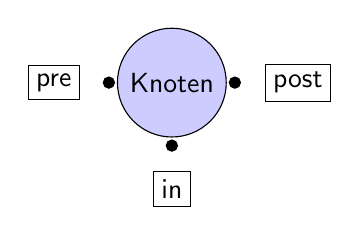
\begin{tikzpicture}[shorten >=1pt, node distance=2cm, auto, 
                    every node/.style={circle, draw, fill=blue!20, font=\sffamily}, 
                    every edge/.style={draw, thick, blue}]
                
                    % Define a single node with no label
                    \node[shape=circle,draw=black] (A) at (0,0) {Knoten}; % Center node
                    
                    % Dots around the node (manually placing them)
                    \node[shape=circle,fill=black,inner sep=0.5mm] at (-0.8, 0) {}; % Left dot
                    \node[shape=circle,fill=black,inner sep=0.5mm] at (0.8, 0) {};  % Right dot
                    \node[shape=circle,fill=black,inner sep=0.5mm] at (0, -0.8) {}; % Bottom dot
                    
                    % Text labels without circles
                    \node[shape=rectangle, fill=white, inner sep=1mm] at (-1.5, 0) {pre};   % Left text label
                    \node[shape=rectangle, fill=white, inner sep=1mm] at (0, -1.35) {in};     % Bottom text label
                    \node[shape=rectangle, fill=white, inner sep=1mm] at (1.6, 0) {post};    % Right text label
                \end{tikzpicture}
            }
        \end{figure}
        \end{column}
    \end{columns}
\end{frame}

\begin{frame}{Graphentheorie}
    \textbf{Traversierungen}
    \begin{columns}
        \begin{column}{0.5\textwidth}
        \pause
            \begin{itemize}
                \item Pre-Order (W-L-R)
                \begin{itemize}
                    \item 1, 2, 4, 5, 3, 6, 7, 8, 9
                \end{itemize}
            \end{itemize}
            \pause
            \begin{itemize}
                \item In-Order (L-W-R)
                \begin{itemize}
                    \item 4, 2, 5, 1, 6, 3, 8, 7, 9
                \end{itemize}
            \end{itemize}
            \pause
            \begin{itemize}
                \item Post-Order (L-R-W)
                \begin{itemize}
                    \item 4, 5, 2, 6, 8, 9, 7, 3, 1
                \end{itemize}
            \end{itemize}
        \end{column}
        \onslide
        \begin{column}{0.5\textwidth}
            \begin{figure}[h]
            \centering
            \scalebox{0.7}{ % Adjust scale here
                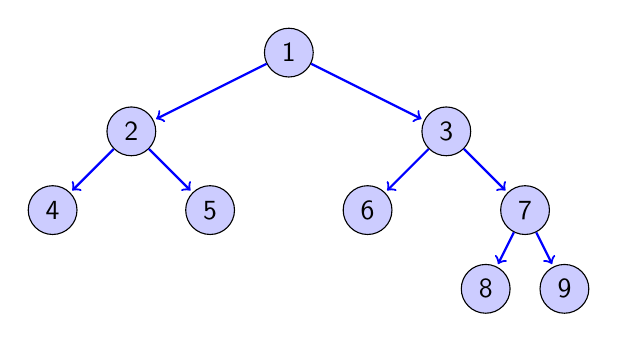
\begin{tikzpicture}[shorten >=1pt, node distance=2cm, auto, 
                    every node/.style={circle, draw, fill=blue!20, font=\sffamily}, 
                    every edge/.style={draw, thick, blue}]
                
                    % Define nodes
                    \node[shape=circle,draw=black] (A) at (0,4) {1}; % Root node
                    \node[shape=circle,draw=black] (B) at (-2,3) {2}; % Child of A
                    \node[shape=circle,draw=black] (C) at (2,3) {3}; % Child of A
                    \node[shape=circle,draw=black] (D) at (-3,2) {4}; % Child of B
                    \node[shape=circle,draw=black] (E) at (-1,2) {5}; % Child of B
                    \node[shape=circle,draw=black] (F) at (1,2) {6}; % Child of C
                    \node[shape=circle,draw=black] (G) at (3,2) {7}; % Child of C
                    \node[shape=circle,draw=black] (H) at (2.5,1) {8}; % Child of G
                    \node[shape=circle,draw=black] (I) at (3.5,1) {9}; % Child of G
        
                    % Define edges
                    \path [->](A) edge (B);
                    \path [->](A) edge (C);
                    \path [->](B) edge (D);
                    \path [->](B) edge (E);
                    \path [->](C) edge (F);
                    \path [->](C) edge (G);
                    \path [->](G) edge (H);
                    \path [->](G) edge (I);
                \end{tikzpicture}
            }
        \end{figure}
        \end{column}
    \end{columns}
\end{frame}

\begin{frame}{Funktionen in Python}
    \pause
    \textbf{Was ist eine Funktion?}
    \pause
    \begin{itemize}
        \item Block an Code der eine bestimmte Aufgabe erfüllt
        \pause
        \item kann Eingabewerte annehmen und einen Ausgabewerte zurückgegeben
    \end{itemize}
    \pause
    \textbf{Vorteile}
    \begin{itemize}
    \pause
        \item Wiederholbarkeit: Codeblock wird \textit{einmal} geschrieben und kann \textit{beliebig} oft aufgerufen werden
        \pause
        \item Lesbarkeit: strukturierter und lesbarer (auch mit sinngemäßen \textit{Funktionsnamen})
        \pause
        \item Modularität: Zerlegen von Logiken eines Programms in leichtere verständlichere Teile
    \end{itemize}
\end{frame}

\begin{frame}{Funktionen in Python}
    \textbf{Kurzes Recap: Die Wichtigeste Typen in Python}
    \begin{itemize}
        \item Text:
        \begin{itemize}
            \item \texttt{str}
        \end{itemize}
        \item Numerisch:
        \begin{itemize}
            \item \texttt{int}, \texttt{float}
        \end{itemize}
        \item Sequenzen:
        \begin{itemize}
            \item \texttt{list}, \texttt{tuple}
        \end{itemize}
        \item Diverse:
        \begin{itemize}
            \item \texttt{dict}, \texttt{set}, \texttt{bool}, \texttt{NoneType}
        \end{itemize}
    \end{itemize}
\end{frame}

\begin{frame}{Funktionen in Python}
    \begin{columns}
        \begin{column}{0.5\textwidth}
            \textbf{Hello-World Funktion}
            \begin{itemize}
                \item einfache Funktion ohne Parameterübergabe oder -rückgabe
                \item Gibt "Hallo Welt!" in der Konsole aus
                \item definiert mit dem \textbf{def} Schlüsselwort
                \pause
                \item aufgerufen wird diese mit \textbf{hello\_world\_func()}
            \end{itemize}
        \end{column}
        \begin{column}{0.5\textwidth}
            \begin{tcolorbox}[colframe=oxfordblue, colback=blue!10, coltitle=white, title=Python]
                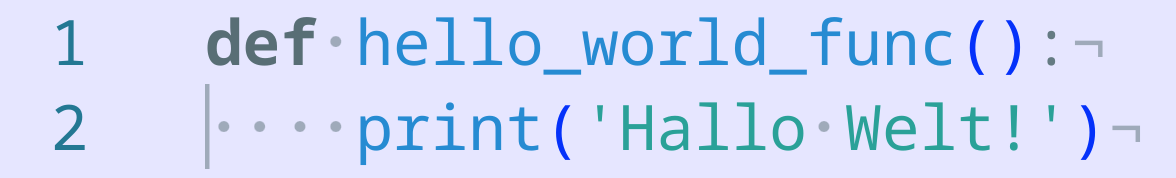
\includegraphics[width=\textwidth]{images/code_helloworldfunction.png}
            \end{tcolorbox}
        \end{column}
    \end{columns}
\end{frame}

\begin{frame}{Funktionen in Python}
    \begin{columns}
        \begin{column}{0.5\textwidth}
            \textbf{Parameterübergabe}
            \begin{itemize}
                \item Variablennamen in den Klammern. mit Komma getrennt, wenn mehrere
                \item \textbf{return} gibt einen Wert zurück
                \item (\textbf{Wichtig: zurückgeben $\neq$ ausgeben})
            \end{itemize}
        \end{column}
        \begin{column}{0.5\textwidth}
            \begin{tcolorbox}[colframe=oxfordblue, colback=blue!10, coltitle=white, title=Python]
                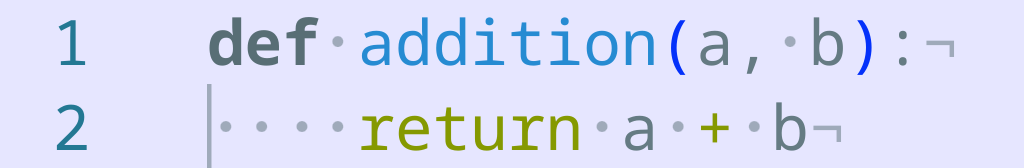
\includegraphics[width=\textwidth]{images/code_inputandreturnfunction.png}
            \end{tcolorbox}
        \end{column}
    \end{columns}
\end{frame}

\begin{frame}{Funktionen in Python}
    \begin{columns}
        \begin{column}{0.5\textwidth}
            \textbf{Standardwerte}
            \begin{itemize}
                \item Fall-Back, falls der geforderte Parameter nicht übergeben wurde
            \end{itemize}
        \end{column}
        \begin{column}{0.5\textwidth}
            \begin{tcolorbox}[colframe=oxfordblue, colback=blue!10, coltitle=white, title=Python]
                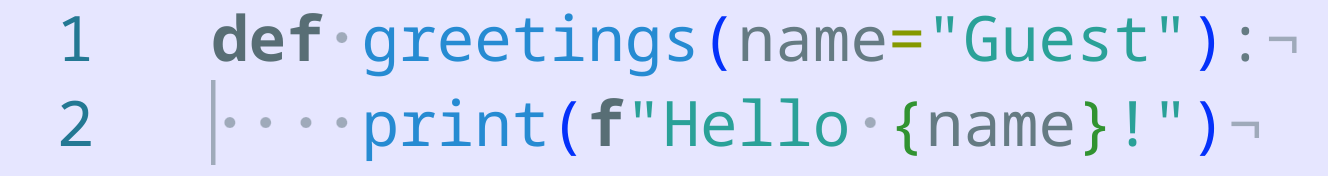
\includegraphics[width=\textwidth]{images/code_fallbackparameterfunction.png}
            \end{tcolorbox}
        \end{column}
    \end{columns}
\end{frame}

\begin{frame}{Funktionen in Python}
    \begin{columns}
        \begin{column}{0.5\textwidth}
            \textbf{Lambda Funktionen}
            \begin{itemize}
                \item Annonyme kurze Funktionen mit \textbf{lambda} Schlüsselwort
            \end{itemize}
        \end{column}
        \begin{column}{0.5\textwidth}
            \begin{tcolorbox}[colframe=oxfordblue, colback=blue!10, coltitle=white, title=Python]
                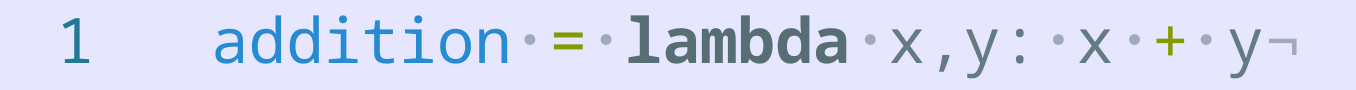
\includegraphics[width=\textwidth]{images/code_lambdafunction.png}
            \end{tcolorbox}
        \end{column}
    \end{columns}
\end{frame}

\begin{frame}{Iteration und Rekursion}
    \textbf{Was ist Iteration?}
    \begin{itemize}
        \item einen bestimmten Codeabschnitt mehrfach ausführen, etwa über eine Schleife (in Python \textbf{for} und \textbf{while}
        \item Häufig um eine iterierbare Datenstruktur zu durchlaufen
    \end{itemize}
\end{frame}

\begin{frame}{Iteration und Rekursion}
    \textbf{Vorteile der Iteration}
    \begin{itemize}
        \item klar und verständlich
        \item gut geeignet wenn Anzahl der Iterationen bekannt
        \item Speichereffizient. wird Schritt für Schritt ausgeführt
    \end{itemize}
\end{frame}

\begin{frame}{Iteration und Rekursion}
    \textbf{Beispiele zur Iteration}
    \vspace{1cm}
    \begin{columns}
        \begin{column}{0.5\textwidth}
            \begin{tcolorbox}[colframe=oxfordblue, colback=blue!10, coltitle=white, title=Python]
                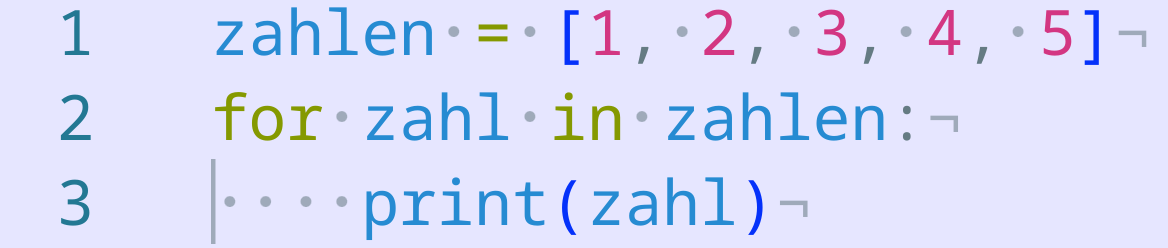
\includegraphics[width=\textwidth]{images/code_iterationexamplesimple.png}
            \end{tcolorbox}
        \end{column}
        \pause
        \begin{column}{0.5\textwidth}
            \begin{tcolorbox}[colframe=oxfordblue, colback=blue!10, coltitle=white, title=Python]
                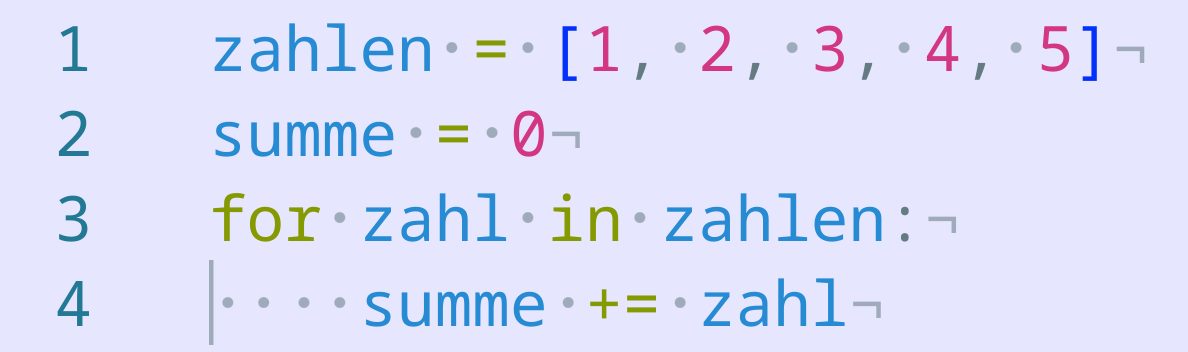
\includegraphics[width=\textwidth]{images/code_iterationsumnumbers.png}
            \end{tcolorbox}
        \end{column}
    \end{columns}
    \vspace{1cm}
\end{frame}

\begin{frame}{Iteration und Rekursion}
    \textbf{Was ist Rekursion?}
    \begin{itemize}
        \item eine Funktion ruft sich selbst solange auf, bis eine Abbruchbedingung erfüllt ist.
        \pause
        \item Das Problem wird in kleinere Teilprobleme unterteilt, die einfacher zu lösen sind
        \pause
        \item Nach dem Erfüllen der Abbruchbedingung ist das Problem gelöst und der erziehlte Wert kann zurückgegeben werden
        \pause
        \item Besteht aus:
        \begin{itemize}
            \item Mindestens einem Basisfall: beendet den Rekursionszweig
            \item Rekursionsfälle: führt zu weiteren rekursiven Aufrufen mit modifizierten Argumenten
        \end{itemize}
    \end{itemize}
\end{frame}

\begin{frame}{Iteration und Rekursion}
    \textbf{Vorteile der Rekursion}
    \begin{itemize}
        \item kann Probleme eleganter und kürzer lösen (generell nur bei Rekursiven Problemen wie z.B. \textit{Fibonacci}, \textit{Baumdurchläufe}, etc...)
    \end{itemize}
    \pause
    \textbf{Nachteile der Rekursion}
    \begin{itemize}
        \item kann zu hoher Speicherauslastung führen, vor allem wenn edge cases zu lasch definiert oder Eingabewerte zu groß sind
        \item Rekursive Lösungen sind in einigen Fällen weniger effizient als iterative
    \end{itemize}
\end{frame}

\begin{frame}{Iteration und Rekursion}
    \textbf{Rekursionsarten}
    \begin{itemize}
        \item Lineare Rekursion
        \item Baumrekursion
        \item Wechselseitige Rekursion
        \item Endrekursion \textit{(Spezialfall der linearen Rekursion)}
    \end{itemize}
\end{frame}

\begin{frame}{Iteration und Rekursion}
    \textbf{Lineare Rekursion}
    \begin{columns}
        \begin{column}{0.5\textwidth}
            \begin{itemize}
                \item Im Rekursionsfall wird die Funktion genau ein Mal aufgerufen
            \end{itemize}
        \end{column}
        \pause
        \begin{column}{0.5\textwidth}
            \begin{tcolorbox}[colframe=oxfordblue, colback=blue!10, coltitle=white, title=Python]
                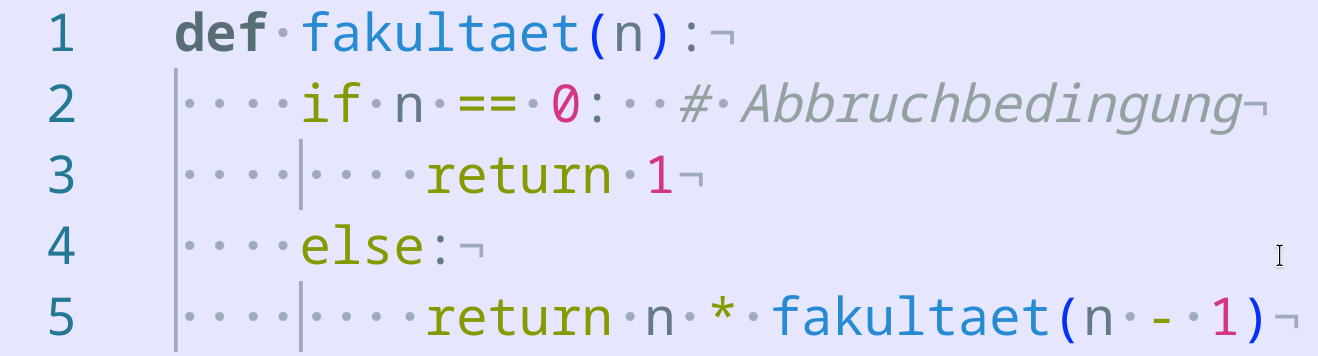
\includegraphics[width=\textwidth]{images/code_recursionfacultyexample.png}
            \end{tcolorbox}
        \end{column}
    \end{columns}
\end{frame}

\begin{frame}{Iteration und Rekursion}
    \textbf{Baumrekursion}
    \begin{columns}
        \begin{column}{0.5\textwidth}
            \begin{itemize}
                \item Im Rekursionsfall wird die Funktion \textbf{mehr} als ein Mal aufgerufen
            \end{itemize}
        \end{column}
        \pause
        \begin{column}{0.5\textwidth}
            \begin{tcolorbox}[colframe=oxfordblue, colback=blue!10, coltitle=white, title=Python]
                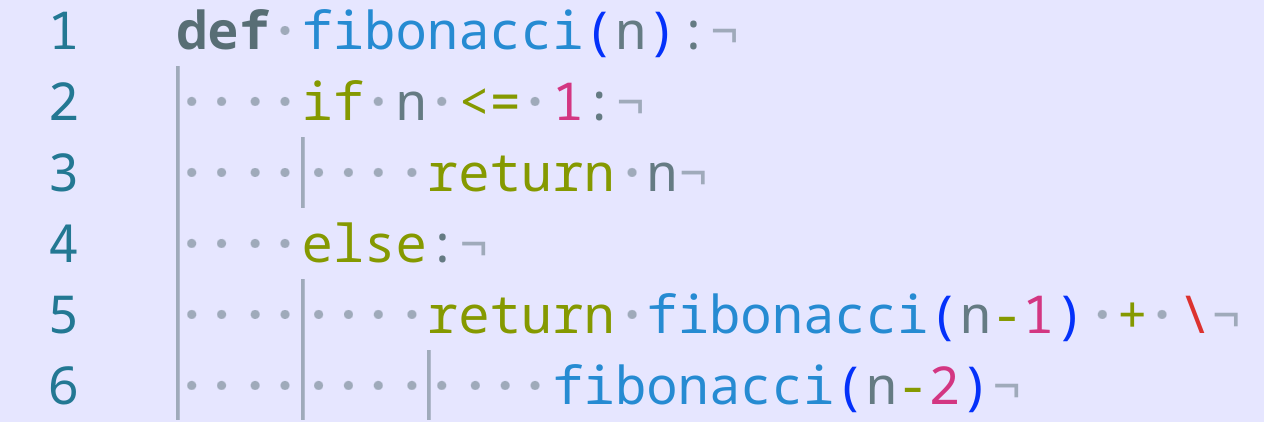
\includegraphics[width=\textwidth]{images/code_recursionfibonacci.png}
            \end{tcolorbox}
        \end{column}
    \end{columns}
\end{frame}

\begin{frame}{Iteration und Rekursion}
    \textbf{Wechselseitige Rekursion}
    \begin{columns}
        \begin{column}{0.5\textwidth}
            \begin{itemize}
                \item Mindestens zwei Funktionen sind im Rekursionsfall jeweils über die andere Funktion definiert
            \end{itemize}
        \end{column}
        \pause
        \begin{column}{0.5\textwidth}
            \begin{tcolorbox}[colframe=oxfordblue, colback=blue!10, coltitle=white, title=Python]
                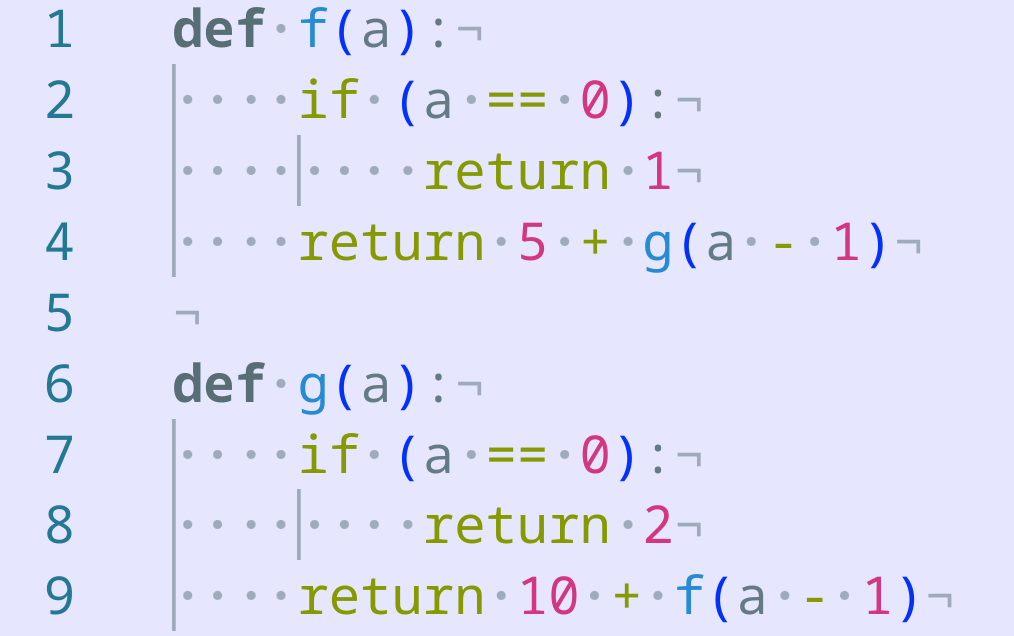
\includegraphics[width=\textwidth]{images/code_wechselrecursion.png}
            \end{tcolorbox}
        \end{column}
    \end{columns}
\end{frame}

\begin{frame}{Iteration und Rekursion}
    \textbf{Endrekursion}
    \begin{itemize}
        \item Spezialfall der linearen Rekursion
        \item Beim Aufruf der nächsten Rekursion sind alle Berechnungen der aktuellen Funktions-Instanz abgeschlossen
        \item Verbraucht in den meisten Fällen weniger Speicher
    \end{itemize}
\end{frame}

\begin{frame}{Numpy und Pandas}
\textbf{Was ist NumPy?}
    \begin{itemize}
        \item eine Bibliothek für effiziente numerische Berechnungen in Python.
        \item Ermöglicht Arbeiten mit mehrdimensionalen Arrays und Matrizen.
        \item Bietet viele mathematische Funktionen.
    \end{itemize}
\end{frame}

\begin{frame}{Numpy und Pandas}
    \textbf{Erstellen eines Arrays}
    \begin{columns}
        \begin{column}{0.5\textwidth}
            \begin{itemize}
                \item Ein NumPy-Array kann aus einer Liste erstellt werden
            \end{itemize}
            \begin{tcolorbox}[colframe=oxfordblue, colback=blue!10, coltitle=white, title=Python]
                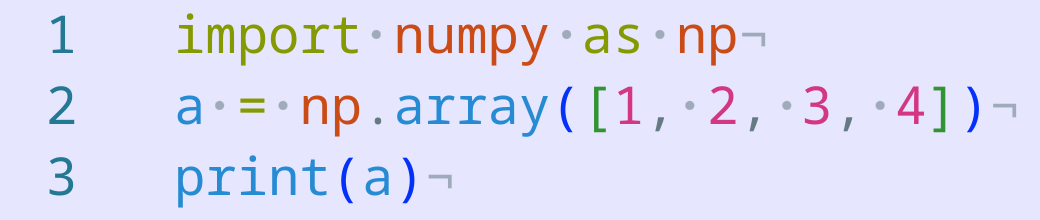
\includegraphics[width=\textwidth]{images/code_numpylistcreation.png}
            \end{tcolorbox}
        \end{column}
        \pause
        \begin{column}{0.5\textwidth}
            \begin{itemize}
                \item Mehrdimensionale Arrays sind ebenfalls möglich
            \end{itemize}
            \begin{tcolorbox}[colframe=oxfordblue, colback=blue!10, coltitle=white, title=Python]
                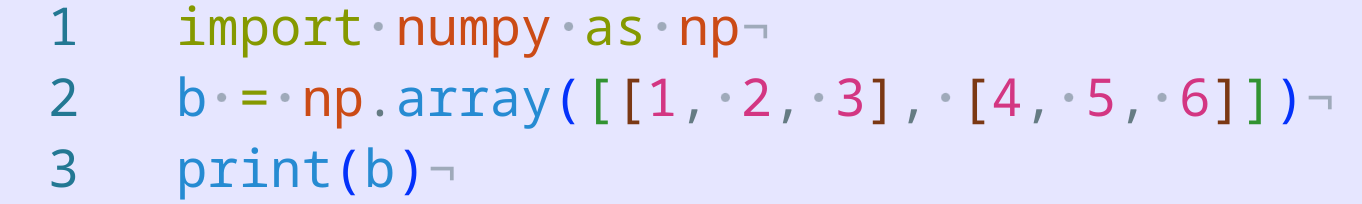
\includegraphics[width=\textwidth]{images/code_numpylistmultidimgeneration.png}
            \end{tcolorbox}
        \end{column}
    \end{columns}
\end{frame}

\begin{frame}{Numpy und Pandas}
    \textbf{Grundlegende Operationen}
    \begin{columns}
        \begin{column}{0.5\textwidth}
            \begin{itemize}
                \item Elementweise Addition
            \end{itemize}
            \begin{tcolorbox}[colframe=oxfordblue, colback=blue!10, coltitle=white, title=Python]
                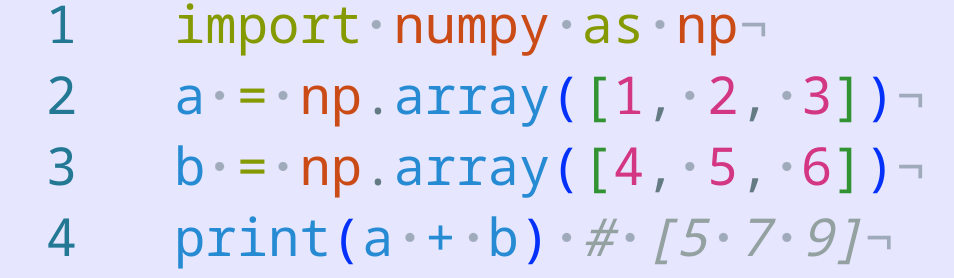
\includegraphics[width=\textwidth]{images/code_numpyelementwiseoperation.png}
            \end{tcolorbox}
        \end{column}
        \pause
        \begin{column}{0.5\textwidth}
            \begin{itemize}
                \item Skalarmultiplikation
            \end{itemize}
            \begin{tcolorbox}[colframe=oxfordblue, colback=blue!10, coltitle=white, title=Python]
                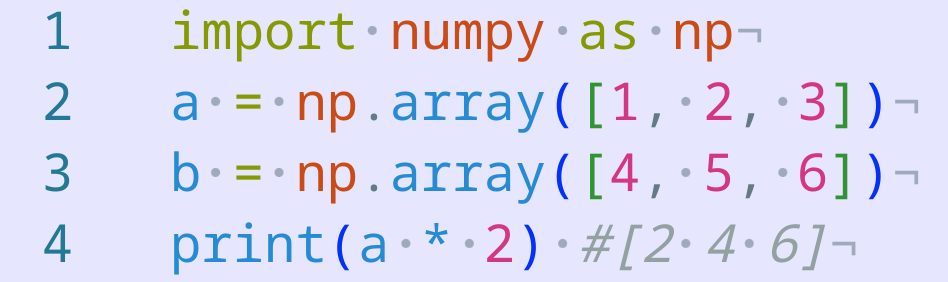
\includegraphics[width=\textwidth]{images/code_numpyscalarproduct.png}
            \end{tcolorbox}
        \end{column}
    \end{columns}
\end{frame}

\begin{frame}{Numpy und Pandas}
    \textbf{Weitere nützliche Funktionen I}
    \begin{tcolorbox}[colframe=oxfordblue, colback=blue!10, coltitle=white, title=Python]
    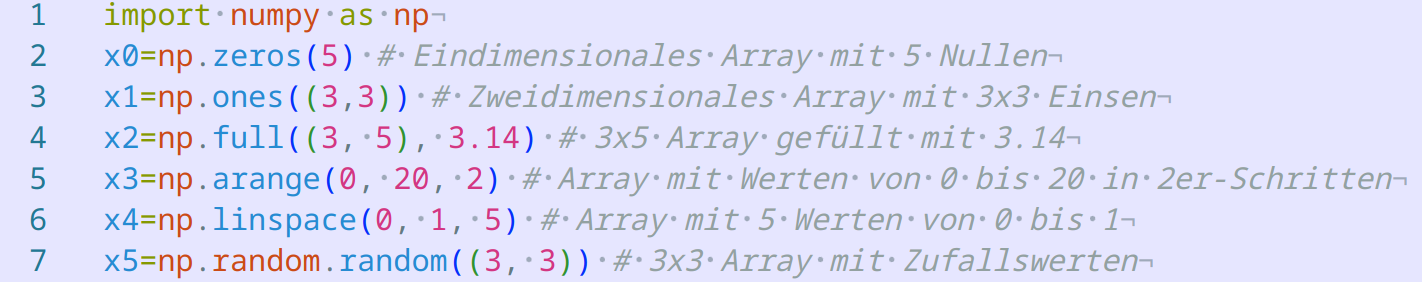
\includegraphics[width=\textwidth]{images/code_numpyusefulfunctions.png}
\end{tcolorbox}
\end{frame}

\begin{frame}{Numpy und Pandas}
    \textbf{Weitere nützliche Funktionen II}
    \begin{columns}
        \begin{column}{0.5\textwidth}
            \begin{tcolorbox}[colframe=oxfordblue, colback=blue!10, coltitle=white, title=Python]
                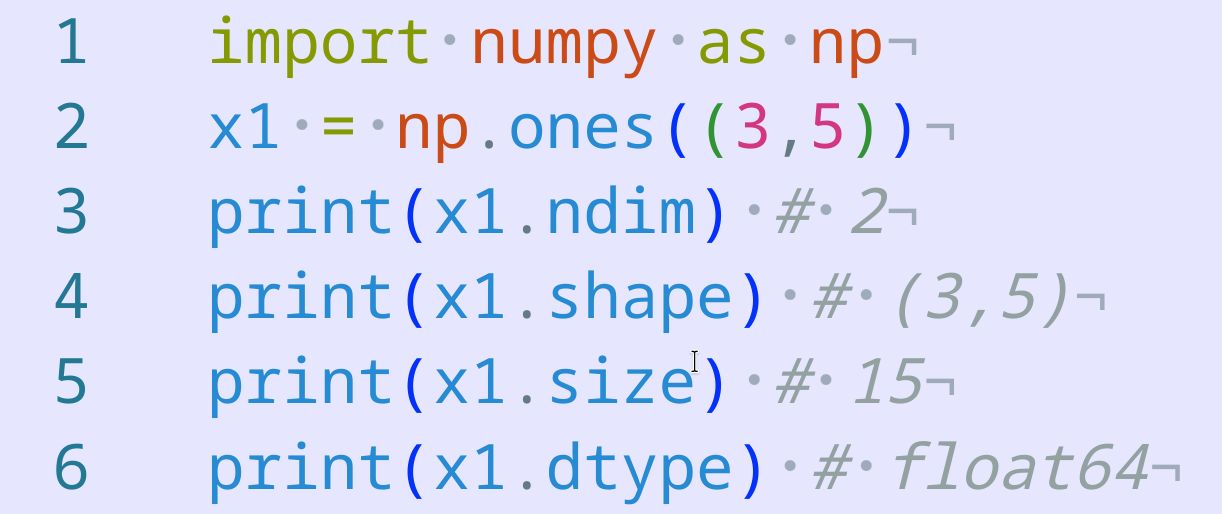
\includegraphics[width=\textwidth]{images/code_numpyothercommands.png}
            \end{tcolorbox}
        \end{column}
        \begin{column}{0.5\textwidth}
            \begin{itemize}
                \item \textbf{ndim}: Anzahl an Dimensionen
                \item \textbf{shape}: Dimensionen z.b. (n,m)
                \item \textbf{size}: Anzahl an Elementen
                \item \textbf{dtype}: Typ der Elemente im Array
            \end{itemize}
        \end{column}
    \end{columns}
    
\end{frame}

\begin{frame}{Numpy und Pandas}
    Das war jetzt nur eine Übersicht der wichtigesten Befehle, zur Klausurvorbereitung sind folgende wichtig:
    \begin{itemize}
        \item EPR Blatt 09
        \item \href{https://realpython.com/numpy-tutorial/}{https://realpython.com/numpy-tutorial/} (sehr ausführlich aber bis zur hälfte etwa Klausurrelevant
    \end{itemize}
\end{frame}

\begin{frame}{Numpy und Pandas}
    \textbf{Was ist Pandas?}
    \begin{itemize}
        \item Pandas ist eine Bibliothek für Datenanalyse und -manipulation.
        \item Bietet Datenstrukturen wie DataFrame und Series.
        \item Erleichtert das Laden, Bearbeiten und Analysieren von Daten.
        \pause
        \item Daten werden in sogenannten \textit{Dataframes} gespeichert, in denen sie mit der library leicht analysiert und manipuliert werden können.
    \end{itemize}
\end{frame}

\begin{frame}{Numpy und Pandas}
    \begin{itemize}
        \item Ein DataFrame kann aus einem Dictionary erstellt werden:
    \end{itemize}
    \begin{tcolorbox}[colframe=oxfordblue, colback=blue!10, coltitle=white, title=Python]
        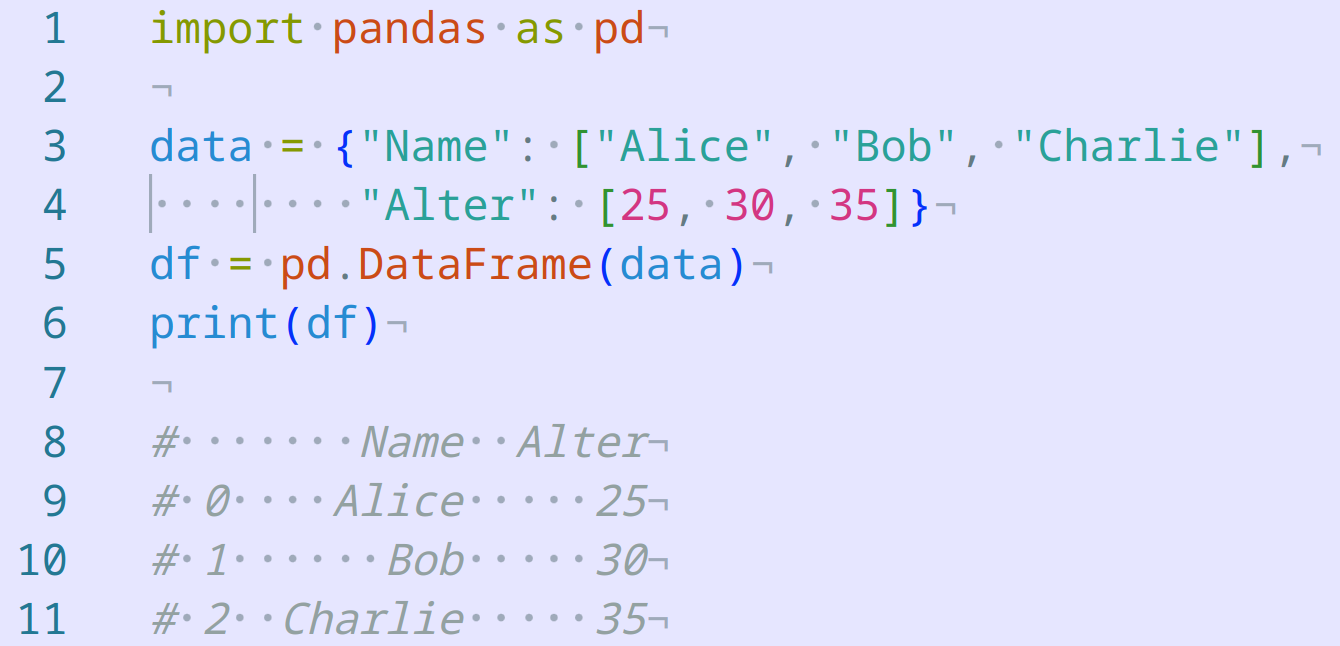
\includegraphics[width=0.7\textwidth]{images/code_pandascreatedataframes.png}
    \end{tcolorbox}
\end{frame}

\begin{frame}{Numpy und Pandas}
    \begin{itemize}
        \item ...oder durch das laden einer CSV-Datei:
    \end{itemize}
    \begin{tcolorbox}[colframe=oxfordblue, colback=blue!10, coltitle=white, title=Python]
        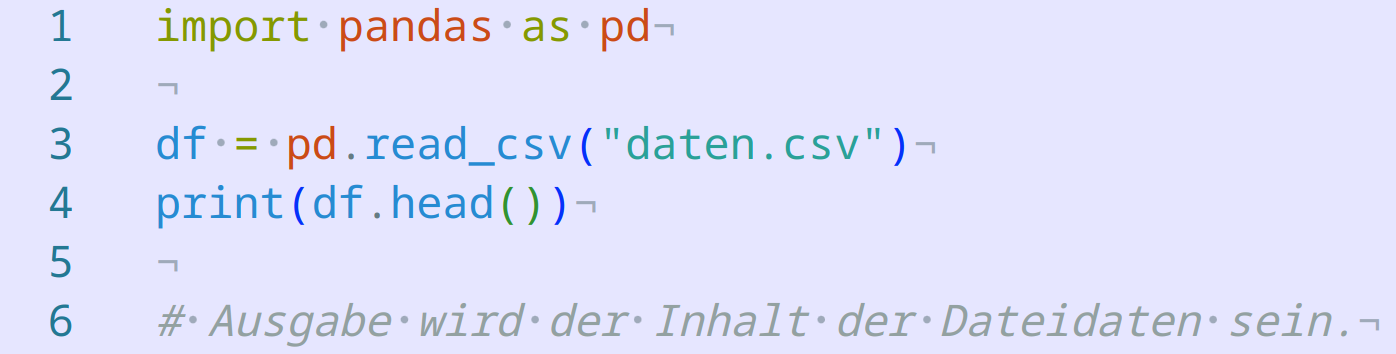
\includegraphics[width=\textwidth]{images/code_pandasdatasetcsv.png}
    \end{tcolorbox}
\end{frame}

\begin{frame}{Numpy und Pandas}
    \begin{itemize}
        \item Zugriff auf Spalten:
    \end{itemize}
    \begin{tcolorbox}[colframe=oxfordblue, colback=blue!10, coltitle=white, title=Python]
        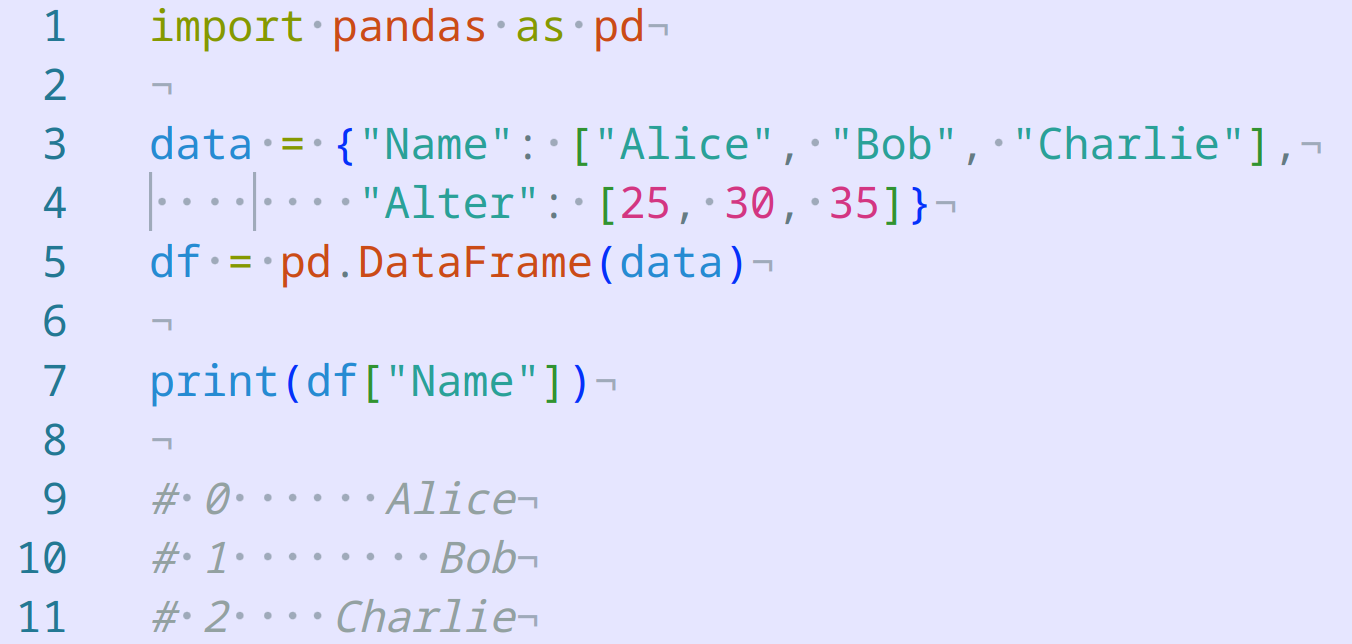
\includegraphics[width=0.7\textwidth]{images/code_pandasfiltercolumn.png}
    \end{tcolorbox}
\end{frame}

\begin{frame}{Numpy und Pandas}
    \begin{itemize}
        \item Filtern von Daten:
        \end{itemize}
    \begin{tcolorbox}[colframe=oxfordblue, colback=blue!10, coltitle=white, title=Python]
        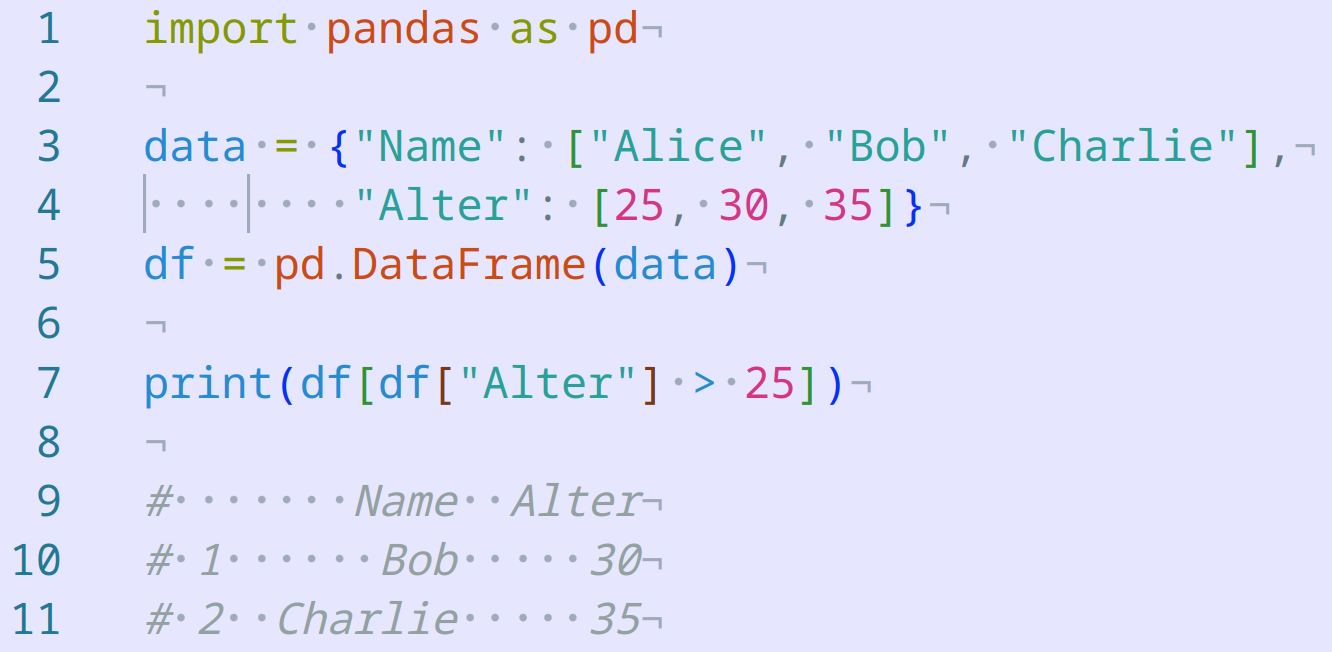
\includegraphics[width=0.65\textwidth]{images/code_pandasfilterdata.png}
    \end{tcolorbox}
\end{frame}

\begin{frame}{Numpy und Pandas}
    \begin{itemize}
        \item Gruppieren von Daten:
        \end{itemize}
    \begin{tcolorbox}[colframe=oxfordblue, colback=blue!10, coltitle=white, title=Python]
        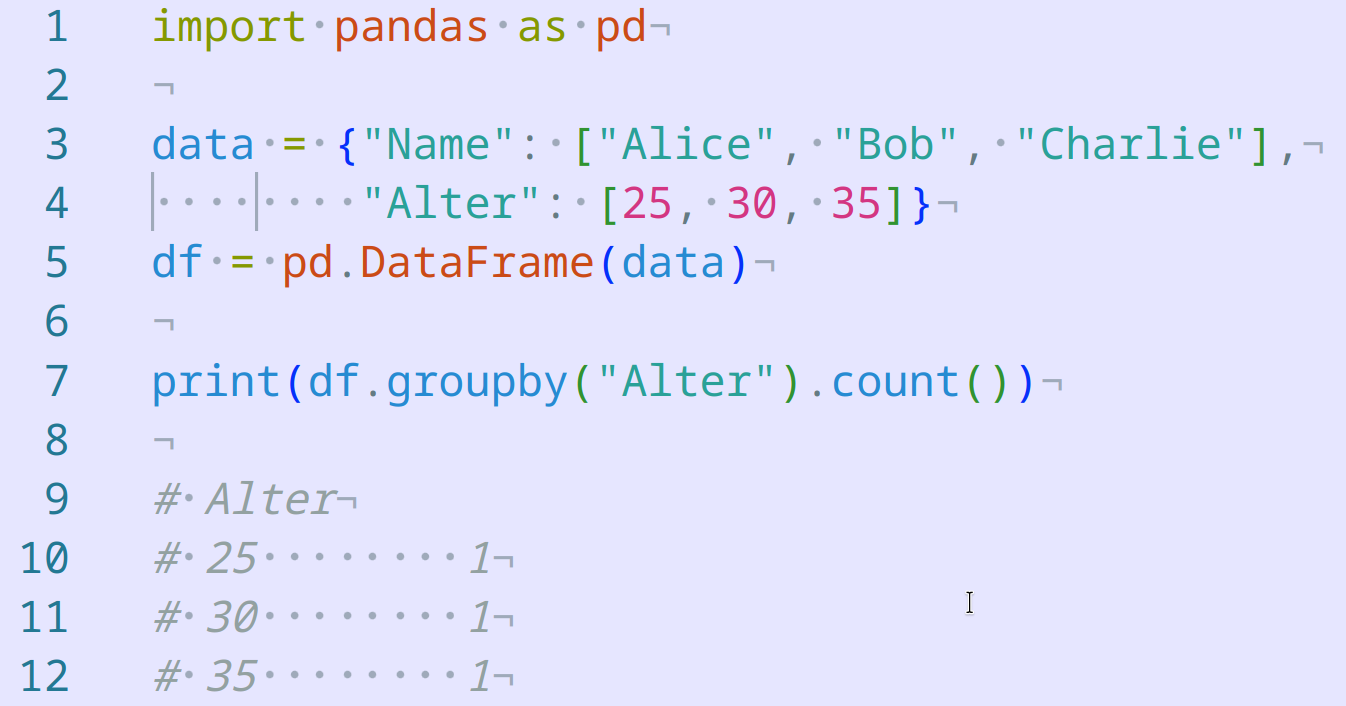
\includegraphics[width=0.6\textwidth]{images/code_pandasgroupadata.png}
    \end{tcolorbox}
\end{frame}

\begin{frame}{Numpy und Pandas}
    \begin{itemize}
        \item Matplotlib ist eine Bibliothek zur Datenvisualisierung.
        \item Beispiel: Erstellen eines einfachen Diagramms:
    \end{itemize}
    \begin{columns}
        \begin{column}{0.5\textwidth}
            \begin{tcolorbox}[colframe=oxfordblue, colback=blue!10, coltitle=white, title=Python]
                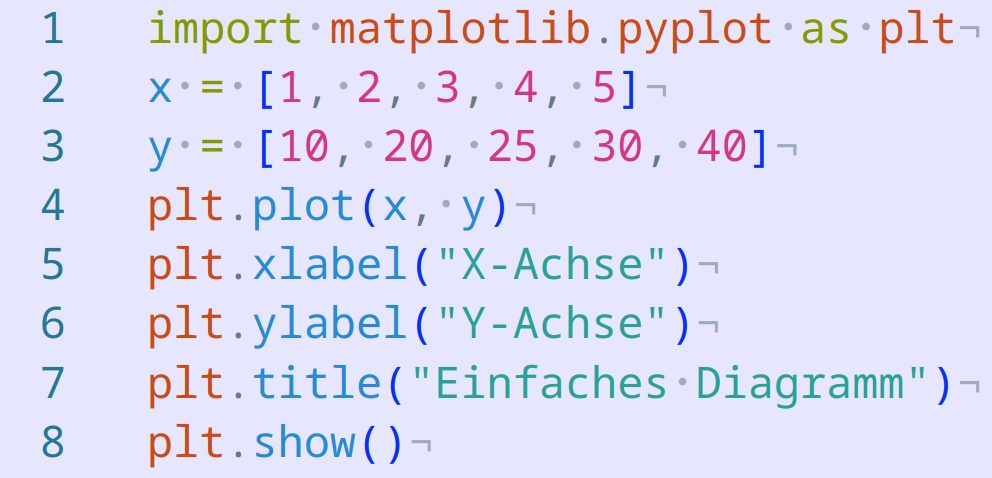
\includegraphics[width=0.9\textwidth]{images/code_matplotlibexample.png}
            \end{tcolorbox}
        \end{column}
        \begin{column}{0.5\textwidth}
            \begin{figure}
                \centering
                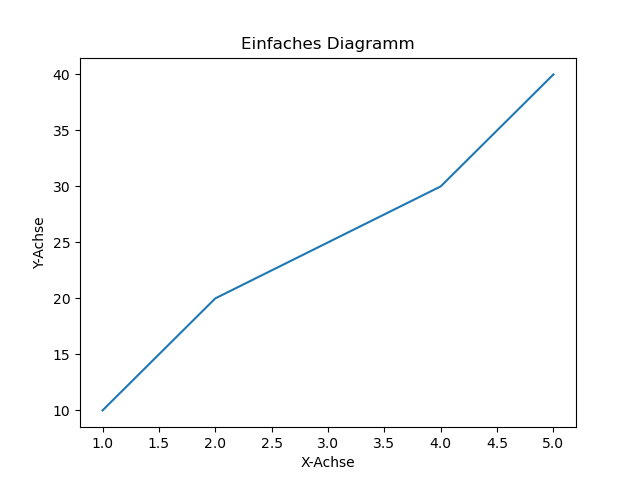
\includegraphics[width=1\linewidth]{images/graph_matplotlibexample.png}
            \end{figure}
        \end{column}
    \end{columns}
\end{frame}

\begin{frame}{Numpy und Pandas}
    \begin{itemize}
        \item Erstellung eines Balkendiagramms aus einem DataFrame:
    \end{itemize}
    \begin{columns}
        \begin{column}{0.5\textwidth}
            \begin{tcolorbox}[colframe=oxfordblue, colback=blue!10, coltitle=white, title=Python]
            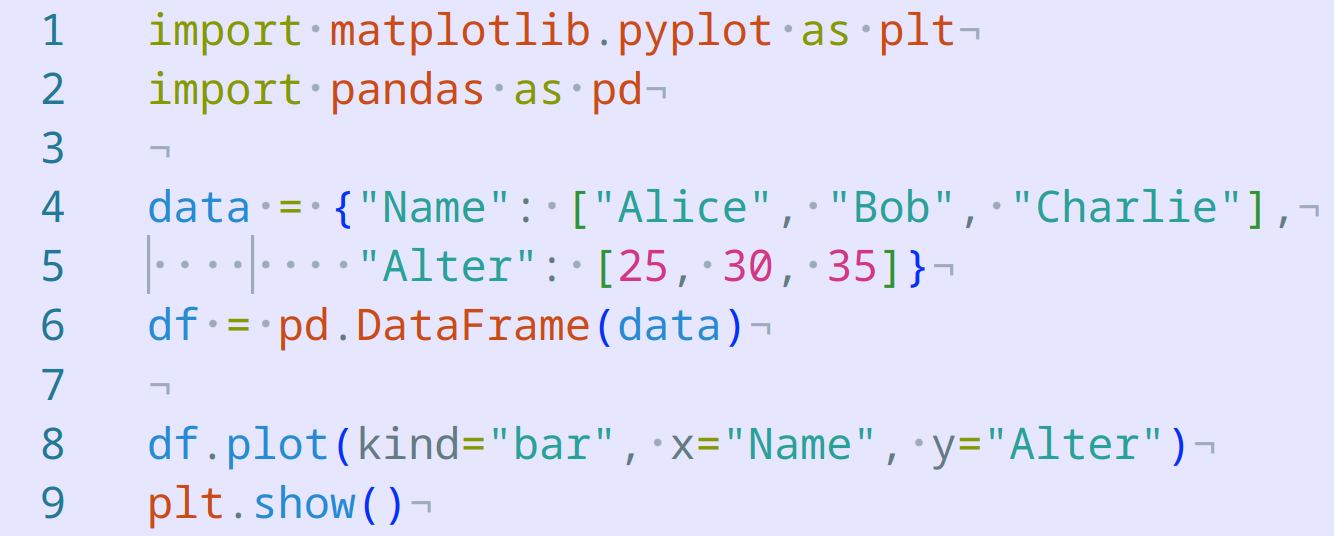
\includegraphics[width=1\textwidth]{images/code_matplotlibpandas.png}
        \end{tcolorbox}
        \end{column}
        \begin{column}{0.5\textwidth}
            \begin{figure}
                \centering
                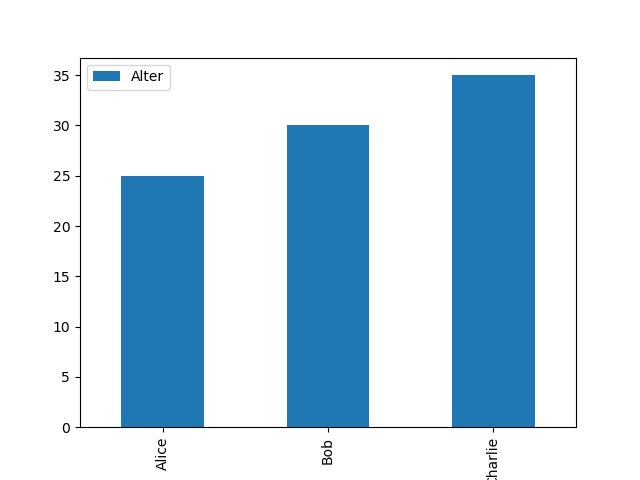
\includegraphics[width=1\linewidth]{images/graph_matplotlibpandas.png}
            \end{figure}
        \end{column}
    \end{columns}
    
\end{frame}

\end{document}
